\documentclass[tikz]{standalone}
\usetikzlibrary{positioning}
\usepackage{xcolor}
\definecolor{processblue}{cmyk}{0.96,0,0,0}
\begin{document}
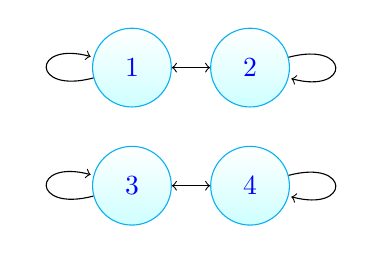
\begin{tikzpicture}[-latex, auto, state/.style={circle, top color=white, bottom color=processblue!20, draw, processblue, text=blue, minimum width=1cm}]
	\node[state] (x) {$1$};
	\node[state] (y) [right of=x, node distance=1.5cm] {$2$};
	\node[state] (z) [below of=x, node distance=1.5cm] {$3$};
	\node[state] (w) [below of=y, node distance=1.5cm] {$4$};
	\path[<->] (x) edge node {} (y);
	\path[<->] (z) edge node {} (w);
	\path[->] (x) edge [loop left] node[left] {} (x);
	\path[->] (y) edge [loop right] node[left] {} (y);
	\path[->] (z) edge [loop left] node[left] {} (z);
	\path[->] (w) edge [loop right] node[left] {} (w);
\end{tikzpicture}
\end{document}